\documentclass{beamer}

% \usepackage[lined,ruled]{algorithm2e}
\usepackage{subfigure}
\usepackage[english]{babel}
\usepackage[latin1]{inputenc}
\usepackage{times}
\usepackage[T1]{fontenc} 
\usepackage{ragged2e}
\usepackage{hyperref}
\usepackage{multimedia}

\usepackage{listings}
\usepackage{algorithm}
\usepackage{algpseudocode}
\usepackage{paralist}

\usepackage{color}
\definecolor{dkgreen}{rgb}{0,0.6,0}
\definecolor{gray}{rgb}{0.5,0.5,0.5}
\definecolor{mauve}{rgb}{0.58,0,0.82}
 
% Default settings for code listings
\lstset{frame=tb,
  language=scala,
  aboveskip=3mm,
  belowskip=3mm,
  showstringspaces=false,
  columns=flexible,
  basicstyle={\small\ttfamily},
  numbers=left,
  numberstyle=\tiny\color{gray},
  keywordstyle=\color{blue},
  commentstyle=\color{dkgreen},
  stringstyle=\color{mauve},
  frame=single,
  breaklines=true,
  breakatwhitespace=true
  tabsize=3
}


\usetheme[secheader]{Boadilla}
\usefonttheme[onlylarge]{structurebold}
\setbeamerfont*{frametitle}{size=\normalsize,series=\bfseries}
\setbeamertemplate{navigation symbols}{}
\setbeamertemplate{mini frames}[box]
\setbeamertemplate{sections/subsections in toc}[square]
\setbeamertemplate{blocks}[rounded][shadow=true]
\setbeamertemplate{bibliography item}[text]

\setbeamercolor{lightorange}{fg=black,bg=orange!40}
\setbeamercolor{lightblue}{fg=black,bg=blue!30}

\newenvironment{colorblock}[2]
{\setbeamercolor{item}{fg=#1,bg=#1}\begin{beamerboxesrounded}[upper=#1,lower=#2,shadow=true]}
  {\end{beamerboxesrounded}}


% Setup TikZ
\usepackage{tikz}
\usetikzlibrary{arrows}
\tikzstyle{block}=[draw opacity=0.7,line width=1.4cm]


%%%%%%%%%%%%%%%%%%%%%%%%%%%%%%%%%%%%%
%%%%%%%%%%%%%%%%%%%%%%%%%%%%%%%%%%%%%
%%%%%%%%%%%%%%%%%%%%%%%%%%%%%%%%%%%%%

\newtheorem{observation}[theorem]{Observation} 

%%%%%%%%%%%%%%%%%%%%%%%%%%%%%%%%%%%%%
%%%%%%%%%%%%%%%%%%%%%%%%%%%%%%%%%%%%%
%%%%%%%%%%%%%%%%%%%%%%%%%%%%%%%%%%%%%

\title{Ethics for Data Scientists}
% \subtitle{}
\author{Paul Pidou}
\institute{EURECOM}
\date


\begin{document}

\begin{frame}
  \titlepage
\end{frame}

%%%%%%%%%%%%%%%%%%%%%%%%%%%%%%%%%%%%%%%%%%%%%%%%%%%
\section{Overview}

\begin{frame}
 \begin{colorblock}{blue}{lightblue}{ }
  \begin{center}
    \Huge \textbf{\texttt{Overview}}
  \end{center}
  \end{colorblock}
\end{frame}

\begin{frame}\frametitle{Scope of the class}
\begin{itemize}
	\setlength\itemsep{1em}
	\item {\bf This class is about:}
	\begin{itemize}
		\item The social responsibility of Data Scientists
		\item Data \& Model validity
		\item The need for a Code of Ethics for Data Scientists
	\end{itemize}	
	\item {\bf This class is NOT about:}
	\begin{itemize}
		\item Laws: legality doesn't imply ethicality
		\item Philosophy: we will not dive into complex notions of ethics
	\end{itemize}
\end{itemize}

\vspace{2em}
\justifying
In a nutshell, this class is a simple framework for thinking about the societal impact of a Data Scientist's job
\end{frame}

%%%%%%%%%%%%%%%%%%%%%%%%%%%%%%%%%%%%%%%%%%%%%%%%%%%
\section{Introduction}

\begin{frame}
 \begin{colorblock}{blue}{lightblue}{ }
  \begin{center}
    \Huge \textbf{\texttt{Introduction}}
  \end{center}
  \end{colorblock}
\end{frame}

\begin{frame}\frametitle{Need for Codes of Ethics \& regulations through history}
\begin{itemize}
	\setlength\itemsep{1em}
	\item {\bf Birth of modern journalism ethics}
	\begin{itemize}
		\item As modern journalism takes over, its role in a democracy has been heavily debated
		\item Journalists have a role of mediator between the general public and policy-making elites
		\item A Code of Ethics of the profession appeared and evolved over time
	\end{itemize}
	\item {\bf Industrial Revolution}
	\begin{itemize}
		\item First industrial revolution started in the late 17\textsuperscript{th} century
		\item Second industrial revolution followed in the mid-19\textsuperscript{th} century
		\item Increased use of coal, petroleum \& chemicals
		\item First Clean Air Act (US) was enacted in 1955
		\item Kyoto Protocol was signed in 1997 and is effective since 2005
	\end{itemize}
\end{itemize}
\begin{center}
{\bf Codes of Ethics} and {\bf regulations} appear after domains emerged and evolved with them
\end{center}
\end{frame}

\begin{frame}\frametitle{Information Revolution}
\begin{itemize}
	\setlength\itemsep{1em}
	\item {\bf Most of the data in the world today has been created in the last few years alone}
	\begin{itemize}
		\item It is a major shift in the relationship we have with our environment
	\end{itemize}
	\item {\bf It is now easier to collect data than ever before}
	\begin{itemize}
		\item People are the producers and/or the consumers of those data
		\item Data are fundamentally about people
	\end{itemize}
	\item {\bf Who owns the data?} (e.g. if I take a picture of you)
	\item {\bf Sense of responsibilities: call for a \textit{Hippocratic Oath}}
\end{itemize}
\end{frame}

\begin{frame}\frametitle{What are Ethics?}
\begin{itemize}
	\item {\bf Ethics are not about laws}
	\begin{itemize}
		\item It is about what we, as society, think is right
		\item Laws are somehow used to enforce ethical behavior
	\end{itemize}
\end{itemize}
\begin{block}{Ethics in a nutshell}
Ethics are our shared social values. Those values lead to shared rules that we all agree to follow because of the resulting benefits.
\end{block}
{\bf Illustration with the \textit{Tragedy of the Commons}}\\
\justifying
Economic theory of a situation within a shared-resource system where individual users acting independently according to their own self-interest behave contrary to the common good of all users by depleting or spoiling that resource through their collective action.
\end{frame}

%%%%%%%%%%%%%%%%%%%%%%%%%%%%%%%%%%%%%%%%%%%%%%%%%%%
\section{Informed consent, Privacy \& Anonymity}

\begin{frame}
 \begin{colorblock}{blue}{lightblue}{ }
  \begin{center}
    \Huge \textbf{\texttt{Informed consent, Privacy \& Anonymity}}
  \end{center}
  \end{colorblock}
\end{frame}

\begin{frame}\frametitle{Informed Consent}
\begin{block}{Definition}
\justifying
Informed consent is a legal procedure to ensure that a patient, client and research participants are aware of all the potential risks and costs involved in a treatment or procedure.
\end{block}
\begin{itemize}
	\setlength\itemsep{1em}
	\item {\bf Common to accept multiple pages of \textit{Terms of Service} when you use a new service}
	\begin{itemize}
		\item Useful from a legal point of view
		\item All-or-nothing choice, no granularity generally
		\item It is really a choice in the first place?
		\begin{itemize}
			\item e.g. Is owning a cellphone still a choice today?
		\end{itemize}
	\end{itemize}
\end{itemize}
\end{frame}

\begin{frame}\frametitle{Facebook's mood experiment}
\begin{itemize}
	\setlength\itemsep{1em}
	\item In 2014, {\bf Facebook} conducted an experiment on 689,003 users without informing them that it was manipulating their \textit{News Feed}
	\begin{itemize}
		\item It was surely legal but was it ethical?
	\end{itemize}
\end{itemize}
\vspace{1em}
Original paper: \textit{Experimental evidence of massive-scale emotional contagion through social networks}
\begin{block}{Significance}
\justifying
We show, via a massive (N = 689,003) experiment on Facebook, that emotional states can be transferred to others via emotional contagion, leading people to experience the same emotions without their awareness. [...]
\end{block}
\end{frame}

\begin{frame}\frametitle{Data Usage Policies \& Restrictions}
\begin{itemize}
	\setlength\itemsep{1em}
	\item {\bf Prospective data collection vs Retrospective data analysis}
	\begin{itemize}
		\item In the first case you are able to inform that will be the usage of the data when you collect them
		\item In the second case you are performing analysis on already collected data
		\item Repurposing is often necessary (e.g. medical data)
	\end{itemize}
	\item {\bf Data usage limitations are necessary}
	\begin{itemize}
		\item Usage of already collected data is not fundamentally bad
		\item Your opinion on how your data can be used can change over time
		\item More granularity on how one can use your data should be the norm
	\end{itemize}
\end{itemize}
\end{frame}

\begin{frame}\frametitle{Privacy}
\begin{itemize}
	\item {\bf Privacy is a basic need}
	\begin{itemize}
		\item Even for people who have "nothing to hide"
		\item Privacy is {\bf not} complete non-disclosure
		\item Privacy is choosing with whom you want to share your data
	\end{itemize}
\end{itemize}
\begin{block}{Definition}
\justifying
Privacy is the ability of an individual or group to seclude themselves, or information about themselves, and thereby express themselves selectively
\end{block}
\begin{itemize}
	\item {\bf Modern privacy risks}
	\begin{itemize}
		\item Easy to collect and store data, potentially forever
		\item Easy to aggregate \& correlate data
		\begin{itemize}
		\item Business of \textit{Data Brokers}
	\end{itemize}
	\end{itemize}
\end{itemize}
\end{frame}

\begin{frame}\frametitle{Target \& the pregnant teenager}
\begin{itemize}
	\setlength\itemsep{1em}
	\item {\bf Target, a US retailer, is performing analytics on customer purchases}
	\begin{itemize}
		\item For instance, Target is able to figure out if you have a baby on the way by looking at your purchases
		\item In order to keep the future parents as loyal customers it sends them coupons for baby items
		\item In 2012, an article from Forbes tells the story of a father learning that his teen daughter was pregnant through Target coupons
		\item Can be seen as an intrusion into privacy
		\item Aware of this issue, Target now sends mixed ads
		\begin{itemize}
			\item The idea is to pretend it knows less than it actually does so as not to create unease 
		\end{itemize}
	\end{itemize}
\end{itemize}
N.B.: If you are interested in this type of analysis, you are encouraged to read Chapters 6 \& 9 of \textit{\href{http://www.mmds.org/}{Mining of Massive Datasets}}
\end{frame}

\begin{frame}\frametitle{Right to privacy}
\begin{itemize}
	\setlength\itemsep{1em}
	\item {\bf We are used to privacy by trust}
	\begin{itemize}
		\item We know with whom we are sharing your data (e.g. a doctor)
		\item Exchange of information is symmetric in this case
		\begin{itemize}
			\item In the sense that you know what one can do with your data
		\end{itemize}
	\end{itemize}
	\item {\bf We need to have privacy by design}
	\begin{itemize}
		\item Your data is exchanged between lots of players now
		\item Exchange of information is therefore asymmetric
		\item We have to ensure that privacy is appropriately respected and managed
		\begin{itemize}
			\item There is the \textit{Right to be forgotten} in the EU
		\end{itemize}
	\end{itemize}
\end{itemize}
\end{frame}

\begin{frame}\frametitle{Anonymity}
\begin{block}{Definition}
\justifying
Anonymity is the quality or state of being anonymous, i.e.\ not being named or identified
\end{block}
\begin{itemize}
	\setlength\itemsep{1em}
	\item {\bf Anonymity seems simple to put in place}
	\begin{itemize}
		\item But it can be easy to trace back individuals
		\begin{itemize}
			\item De-identification has limited value
			\item Netflix Prize example
		\end{itemize}
		\item Anonymity is virtually impossible given so many data streams
	\end{itemize}
	\item {\bf As for privacy we need to have anonymity by design}
	\begin{itemize}
		\item License data to trusted parties
		\item Enforce anonymity by contracts and/or professional standards
	\end{itemize}
\end{itemize}
\end{frame}

\begin{frame}\frametitle{The Netflix Prize example}
\begin{block}{The Netflix Prize}
\justifying
It was an open competition for the best collaborative filtering algorithm to predict user ratings for films, based on previous ratings without any other information about the users or films, i.e.\ without the users or the films being identified except by numbers assigned for the contest.
\end{block}
\begin{itemize}
	\setlength\itemsep{1em}
	\item In 2007, Arvind Narayanan and Vitaly Shmatikov, researchers at the University of Texas, published a paper called \textit{Robust De-anonymization of Large Sparse Datasets}
	\item They successfully de-anonymized some of the Netflix data by comparing rankings and timestamps with public information in the Internet Movie Database (IMDb)
\end{itemize}
\end{frame}

\begin{frame}\frametitle{The Netflix Prize example (cont'd)}
\begin{itemize}
	\setlength\itemsep{1em}
	\item Their idea was fairly simple: when a Netflix user finishes watching a movie, he is likely to rate it on IMDb
	\begin{itemize}
		\item The timestamps and the ratings between the two websites are likely to be close
		\item Thanks to IMDb accounts they were able to find back some of the individuals behind the Netflix ones
	\end{itemize}
	\item You might wonder: \textit{but what is the issue? People purposely displayed on IMDb the movies they watched right?}
	\begin{itemize}
		\item The issue is that they displayed \textit{some} of the movies they watched on Netflix but not \textit{all} of them
		\item We are back to {\bf privacy} issues where users' data are displayed and used without their fully {\bf informed consent}
	\end{itemize}
\end{itemize}
\end{frame}

%%%%%%%%%%%%%%%%%%%%%%%%%%%%%%%%%%%%%%%%%%%%%%%%%%%
\section{Data \& Models validity}

\begin{frame}
 \begin{colorblock}{blue}{lightblue}{ }
  \begin{center}
    \Huge \textbf{\texttt{Data \& Models validity}}
  \end{center}
  \end{colorblock}
\end{frame}

\begin{frame}\frametitle{Data validity}
\begin{itemize}
	\setlength\itemsep{1em}
	\item {\bf Data is the most important component}
	\begin{itemize}
		\item Your model could be the best in the world, but if your data is unreliable then so will the result
		\item Bad data/information leads to bad decisions
		\item Unfortunately we often don't have access to the data we require
	\end{itemize}
	\item {\bf Learn more about the field}
	\begin{itemize}
		\item Data does {\bf not} prevent you to study the field you are working on
		\item It enables feature selection
		\begin{itemize}
			\item[] {\bf Simple example}: if you try to predict the probability that an individual has a beard you will discover that taller people are more keen to have beards. As men are taller than women on average the result is obvious i.e. the size alone is not a good feature in this context.
		\end{itemize}
	\end{itemize}
\end{itemize}
\end{frame}

\begin{frame}\frametitle{Data validity (cont'd)}
\begin{itemize}
	\setlength\itemsep{1em}
	\item {\bf Before to start building a model you have to explore the data}
	\begin{itemize}
		\item Are the data clean?
		\begin{itemize}
			\item Are the continuous values in the range expected?
			\item Are empty fields always marked in the same way?
		\end{itemize}
		\item Are the data really representative of what you want to model?
		\begin{itemize}
			\item If I had to collect data from scratch for a given problem what will I collect?
		\end{itemize}
	\end{itemize}
	\item {\bf Data errors}
	\begin{itemize}
		\item Errors can be of form and substance
		\item Take for granted that there are always form errors in the data
		\begin{itemize}
			\item Form errors: both schema errors and improbable values e.g. due to damaged sensor 
			\item A cleaning pipeline to avoid those errors is necessary
		\end{itemize}
		\item Skewed data
	\end{itemize}
\end{itemize}
\end{frame}

\begin{frame}\frametitle{Skewed data problem}
\begin{itemize}
	\setlength\itemsep{1em}
	\item {\bf Likely in classification problems}
	\begin{itemize}
		\item Classes are possibly not evenly distributed
		\item Leading models to favor some classes over others
		\begin{itemize}
			\item In 2015, Google launched Google Photos that, in Google's words, can automatically tag and label your photos
			\item Google Photos app identified photos of black people as gorillas
		\end{itemize}
	\end{itemize}
	\item {\bf Data are likely biased}
	\begin{itemize}
		\item Data are embedding biases of people who generated and/or collected the data
		\item Data are embedding also societal biases
		\begin{itemize}
			\item Racial biases
			\item Gender biases
		\end{itemize}
	\end{itemize}
\end{itemize}
\end{frame}

\begin{frame}\frametitle{Racial biases}
\begin{itemize}
	\setlength\itemsep{1em}
	\item {\bf Risk assessment software has become increasingly common in courtrooms in the US}
	\begin{itemize}
		\item The system is giving a score to criminals which is supposed to represent the likelihood they will commit a future crime
		\item Those scores are given to judges during criminal sentencing
		\item Those score are heavily biased against black people
		\begin{itemize}
			\item Skin color is not one of the features
			\item Pay attention to features that can serve as proxy
		\end{itemize}
	\end{itemize}
\end{itemize}
\begin{figure}[h]
	\centering
	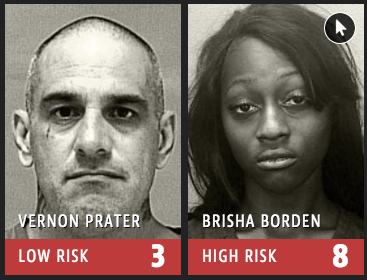
\includegraphics[scale=0.33]{./Figures/risk_assessment}
	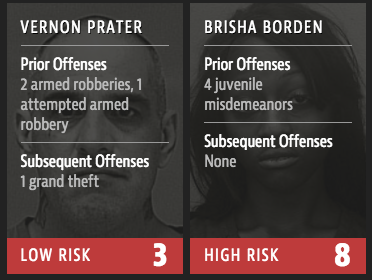
\includegraphics[scale=0.33]{./Figures/risk_assessment2}
	\label{fig:risk_assessment}
\end{figure}
\end{frame}

\begin{frame}\frametitle{Gender biases}
\begin{itemize}
	\setlength\itemsep{1em}
	\item {\bf In Natural Language Processing, one of the most popular systems of word representation is \textit{word2vec}}
	\begin{itemize}
		\item Trained on hundreds of thousands of articles taken from Google News, \textit{word2vec} has been tested to show that it represents the English vocabulary very well
		\item For example, the difference between the vectors "man" and "king" is equal to the difference between the vectors "woman" and "queen"
		\begin{itemize}
			\item Noted as "man: king; woman: queen"
		\end{itemize}
		\item The issue is that some of the relations are questionable
		\begin{itemize}
			\item "father: doctor; mother: nurse"
			\item "man: computer programmer; woman: homemaker"
			\item "she: he; sewing: carpentry"
			\item "she: he; nude: shirtless"
		\end{itemize}
	\end{itemize}
\end{itemize}
N.B.: See the paper \textit{\href{https://arxiv.org/abs/1607.06520}{Man is to Computer Programmer as Woman is to Homemaker? Debiasing Word Embeddings}}
\end{frame}

\begin{frame}\frametitle{Some tips}
\begin{itemize}
	\setlength\itemsep{1em}
	\item {\bf Always explore the data}
	\begin{itemize}
		\item Look for unlikely values and/or classes
		\item Establish whether the data follows some distribution
		\item Observe how classes are distributed
		\item Ask yourself how those data were produced in the first place
	\end{itemize}
	\item {\bf Set up a cleaning pipeline}
	\begin{itemize}
		\item Analyze the repartition of the damaged data accros the different classes
		\item Look if some features can be used as proxy to infer missing ones
		\item Rearrange the data to have evenly distributed classes
		\item Normalize (rescale) the data if needed
		\item Get rid off the too damaged samples
	\end{itemize}
	\item {\bf Study the field and survey the common issues related to it}
\end{itemize}
\end{frame}

\begin{frame}\frametitle{Model validity}
\begin{itemize}
	\setlength\itemsep{1em}
	\item {\bf Model design}
	\begin{itemize}
		\item Even if you have perfect inputs, perfect data, there are many reasons why the model could be incorrect
		\item Most machine learning just estimates parameters to fit a predetermined model
		\item {\bf No Free Lunch theorem}: there is no one ML algorithm that works best all the time, you have to try many of them
	\end{itemize}
	\item {\bf Importance of the model's capacity}
	\begin{itemize}
		\item A model's capacity is its ability to fit a wide variety of functions
		\item Models with low capacity may struggle to fit the training set
		\item Models with high capacity can overfit by memorizing properties of the training set that do not serve them well on the test set
	\end{itemize}
\end{itemize}
\end{frame}

\begin{frame}\frametitle{Model's capacity}
\begin{figure}[h]
	\centering
	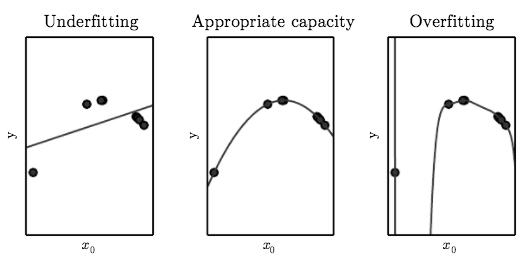
\includegraphics[scale=0.42]{./Figures/model_capacity}
	\label{fig:model_capacity}
\end{figure}
{\bf From left to right}: a linear function, a quadratic function and a polynomial of degree 9

\vspace{1em}
N.B.: Example extracted from \href{http://www.deeplearningbook.org/}{\textit{Deep Learning}, Chapter 5 - Goodfellow}
\end{frame}

\begin{frame}\frametitle{Some tips}
\begin{itemize}
	\setlength\itemsep{1em}
	\item {\bf Keep your model simple}
	\begin{itemize}
		\item Start from a simple model and use it as baseline
		\item Generally, the fewer parameters that you have to tune the better
	\end{itemize}
	\item {\bf Use cross validation}
	\begin{itemize}
		\item Use K-Fold cross validation
		\item According to your dataset you can use Leave One Out Cross Validation (LOOCV)
	\end{itemize}
	\item {\bf Use regularization}
	\begin{itemize}
		\item Add regularizations terms (such as L1, L2, AIC, BIC, MDL or a probabilistic prior) to the objective function
	\end{itemize}
	\item {\bf Pay attention to the objective function you are using}
	\begin{itemize}
		\item It is very important as it will be used to optimize the model
	\end{itemize}
\end{itemize}
\end{frame}

\begin{frame}\frametitle{Don't conclude too fast}
\begin{block}{Simpson's paradox}
\justifying
Simpson's paradox, or the Yule-Simpson effect, is a paradox in probability and statistics, in which a trend appears in different groups of data but disappears or reverses when these groups are combined
\end{block}
\begin{itemize}
	\item {\bf UC Berkeley gender bias example}
	\begin{itemize}
		\item Study of gender bias among graduate school admissions to University of California, Berkeley
		\item Here is the admission figures for the fall of 1973:
		\begin{figure}[h]
			\centering
			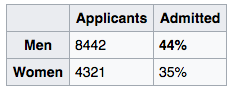
\includegraphics[scale=0.55]{./Figures/ucb_gender1}
			\label{fig:radmission_figures}
		\end{figure}
	\end{itemize}
\end{itemize}
\end{frame}

\begin{frame}\frametitle{UC Berkeley gender bias example (cont'd)}
\justifying
It seems biased in favor of men but when examining the individual departments, it appeared that six out of 85 departments were significantly biased against men, whereas only four were significantly biased against women. Here is the the data from the six largest departments:
\begin{figure}[h]
	\centering
	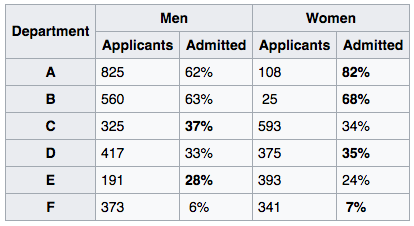
\includegraphics[scale=0.5]{./Figures/ucb_gender2}
	\label{fig:radmission_figures2}
\end{figure}
The \href{http://homepage.stat.uiowa.edu/~mbognar/1030/Bickel-Berkeley.pdf}{research paper by Bickel et al} concluded that women tended to apply to competitive departments (low rates of admission) whereas men tended to apply to less-competitive departments
\end{frame}

\begin{frame}\frametitle{Managing change}
\begin{block}{Campbell's law}
\justifying
It is an adage developed by Donald T. Campbell: "The more any quantitative social indicator is used for social decision-making, the more subject it will be to corruption pressures and the more apt it will be to distort and corrupt the social processes it is intended to monitor."
\end{block}
\begin{itemize}
	\setlength\itemsep{1em}
	\item In other words as stated by the Goodhart's law: "When a measure becomes a target, it ceases to be a good measure."
	\item {\bf Things change over time}
	\begin{itemize}
		\item Your model once put in place can modified the environment from which the initial data came from
		\item People behavior can change over time and therefore your model can become less relevant
		\item You have to monitor the model's efficiency over time
	\end{itemize}
\end{itemize}
\end{frame}

%%%%%%%%%%%%%%%%%%%%%%%%%%%%%%%%%%%%%%%%%%%%%%%%%%%
\section{Societal Impact}

\begin{frame}
 \begin{colorblock}{blue}{lightblue}{ }
  \begin{center}
    \Huge \textbf{\texttt{Societal Impact}}
  \end{center}
  \end{colorblock}
\end{frame}

\begin{frame}\frametitle{Algorithmic fairness}
\begin{itemize}
	\setlength\itemsep{1em}
	\item {\bf We saw that data can be biased}
	\begin{itemize}
		\item If they are not representative of the population
		\item If the past population is not representative of the future population
		\item If confounding processes that lead to correlations are just flukes
	\end{itemize}
	\item {\bf Those data can lead to an algorithmic vicious cycle}
	\begin{itemize}
		\item A bias raises in the algorithm because of the data it is trained on
		\item Once put in place the algorithm perpetuates the bias
		\item Let's say that a company with only 10\% women employees develops a hiring algorithm
		\begin{itemize}
			\item[] The company has a "boys' club culture" that males it difficult for women to succeed. The training algorithm is trained on current data and based on current employee success, it scores the women candidates lower. The algorithm, albeit fairly representing that happens today, perpetuates a gender bias.
		\end{itemize}
	\end{itemize}
\end{itemize}
\end{frame}

\begin{frame}\frametitle{Correct but misleading results}
\begin{itemize}
	\setlength\itemsep{1em}
	\item {\bf Tell a story}
	\begin{itemize}
		\item In your role as a Data Scientist, once you conducted an analysis you are expected to present your results
		\item Visualization is a powerful tool but it can be misleading
		\item You often have to aggregate the results to present them in a more concise way
		\item Your inner biases can lead to highlight specific parts of the results, leading to a specific interpretation of the results
	\end{itemize}
	\item {\bf Diversity suppression}
	\begin{itemize}
		\item Happens when the criteria that an algorithm is using have been been tuned to fit the majority
		\item The algorithm ends up discriminating
		\item Don't rely on accuracy alone: see F-score, type I and type II errors and the tradeoff between precision and recall.
	\end{itemize}
\end{itemize}
\end{frame}

\begin{frame}\frametitle{Unexpected discrimination}
\begin{itemize}
	\setlength\itemsep{1em}
	\item {\bf In 2012, the city of Boston put in place a project called "Street Bump"}
	\begin{itemize}
		\item The idea is to use the accelerometer and the GPS of citizens' smartphones to detect potholes around the city
		\item It is a very good way to use technology to improve citizens' life
		\item Unfortunately, the issue is that it is only working in the areas where people are rich enough to afford a car and a smartphone
		\item The poorer neighborhoods might be underserved
		\item To avoid this, city employees in city vehicles worked to compensate by driving in poorer neighborhoods
	\end{itemize}
	\item {\bf Always step back and think about that could be the consequences of the technology you are putting in place}
	\begin{itemize}
		\item This notion of evaluating the impact is far removed from the every day concerns of data scientists
	\end{itemize}
\end{itemize}
\end{frame}

\begin{frame}\frametitle{Echo chambers / Filter bubbles}
\centering
%\movie[height = 0.6\textwidth, width = 0.8\textwidth, poster, showcontrols]{.Figures/filterbubbles.png}{./media/filterbubbles.mp4} 
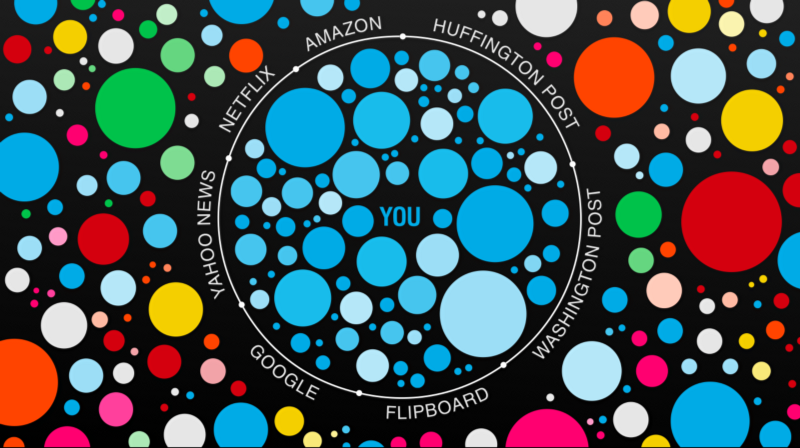
\includegraphics[scale=0.4]{Figures/filterbubbles.png}
\label{figfilter_bubbles}
\href{https://www.ted.com/talks/eli_pariser_beware_online_filter_bubbles}{ted.com/talks/eli\_pariser\_beware\_online\_filter\_bubbles}
\end{frame}


%%%%%%%%%%%%%%%%%%%%%%%%%%%%%%%%%%%%%%%%%%%%%%%%%%%
\section{Conclusion}

\begin{frame}
 \begin{colorblock}{blue}{lightblue}{ }
  \begin{center}
    \Huge \textbf{\texttt{Conclusion}}
  \end{center}
  \end{colorblock}
\end{frame}

\begin{frame}\frametitle{Conclusion}
\begin{itemize}
	\setlength\itemsep{1em}
	\item {\bf We have to accept that algorithms can have biases}
	\begin{itemize}
		\item Due to the data they are based on
		\item Due to people designing the algorithm
		\item Due to the interpretation of the results
	\end{itemize}
	\item {\bf We have to accept that we have inner biases}
	\begin{itemize}
		\item It is only by being aware of it that we can mitigate it
		\item If you have still a doubt about it I invite you to read \textit{The Hidden Brain} from Shankar Vedantam
	\end{itemize}
	\item {\bf A simple Code of Ethics}
	\begin{itemize}
		\item Inform people exactly how you intend to use their data
		\item Own the outcomes
		\begin{itemize}
			\item Is it a valid data analysis?
			\item Is it a fair data analysis?
			\item What are the societal consequences?
		\end{itemize}
	\end{itemize}
\end{itemize}
\end{frame}

%%%%%%%%%%%%%%%%%%%%%%%%%%%%%%%%%%%%%%%%%%%%%%%%%%%
\section{References}

\begin{frame}
 \begin{colorblock}{blue}{lightblue}{ }
  \begin{center}
    \Huge \textbf{\texttt{References}}
  \end{center}
  \end{colorblock}
\end{frame}

\begin{frame}\frametitle{References}
\begin{itemize}
	\item \href{https://courses.edx.org/courses/course-v1:MichiganX+DS101x+1T2017/info}{\color{blue}MichiganX: DS101x Data Science Ethics}
	\item \href{http://www.pnas.org/content/111/24/8788.full}{\color{blue}Experimental evidence of massive-scale emotional contagion through social networks}
	\item \href{https://www.forbes.com/sites/kashmirhill/2012/02/16/how-target-figured-out-a-teen-girl-was-pregnant-before-her-father-did/}{\color{blue}How Target Figured Out A Teen Girl Was Pregnant Before Her Father Did}
	\item \href{https://www.cs.cornell.edu/~shmat/shmat_oak08netflix.pdf}{\color{blue}Robust De-anonymization of Large Sparse Datasets}
	\item \href{https://www.propublica.org/article/machine-bias-risk-assessments-in-criminal-sentencing}{\color{blue}Machine bias: Risk assessments in criminal sentencing}
	\item \href{https://www.technologyreview.com/s/602025/how-vector-space-mathematics-reveals-the-hidden-sexism-in-language/}{\color{blue}How Vector Space Mathematics Reveals the Hidden Sexism in Language}
	\item \href{http://homepage.stat.uiowa.edu/~mbognar/1030/Bickel-Berkeley.pdf}{\color{blue}Sex Bias in Graduate Admissions: Data from Berkeley}
	\item \href{https://www.wired.com/insights/2014/03/potholes-big-data-crowdsourcing-way-better-government/}{\color{blue}Potholes and Big Data: Crowdsourcing Our Way to Better Government}
	\item \href{https://www.ted.com/talks/eli_pariser_beware_online_filter_bubbles}{\color{blue}Eli Pariser: Beware online "filter bubbles"}
\end{itemize}
\end{frame}


\end{document}
